
\chapter{Estudo de caso}\label{chap:estudodecaso}

\section{Universidade Estadual do Sudoeste da Bahia}

A Universidade Estadual do Sudoeste da Bahia está situada na Mesorregião do Centro-Sul Baiano, que é formada pela união de 118 municípios, com 2.478.542 habitantes em uma área de 127.878 km$^{2}$, o que corresponde aproximadamente 22,7\% de todo o território da Bahia.$^{[}$\footnote{Informações retiradas do site Cidade Brasil, Disponível em: \url{https://www.cidade-brasil.com.br/mesorregiao-do-centro-sul-baiano.html}. Acessado em 16 de junho de 2018}$^{]}$ Ela é constituída de três campi, Vitória da Conquista, Jequié e Itapetinga, tendo sede em Vitória da Conquista, local em que foi realizado o estudo de caso, à 510 km da capital Salvador. O município de Vitória da Conquista conta com um território de 3.705,838 km$^{2}$ e uma população com 348.718 habitantes.$^{[}$\footnote{Informações retiradas do site Cidades IBGE, Disponível em: \url{https://cidades.ibge.gov.br/brasil/ba/vitoria-da-conquista}.  Acessado em 16 de junho de 2018}$^{]}$

A UESB, campus de Vitória da Conquista, tornou-se o campo desta pesquisa, pois a mesma é uma ampla consumidora e usuária de equipamentos tecnológicos, possuindo um conjunto de equipamentos, computadores, \textit{switches}, servidores, pontos de acessos para rede sem fio, entre outros dispositivos de informática. Segundo o Roteiro de Diagnóstico Setorial$^{[}$\footnote{Roteiro de Diagnóstico Setorial, Disponível em: \url{http://www2.uesb.br/wp-content/uploads/2018/05/UINFOR.pdf}.  Acessado em 16 de junho de 2018}$^{]}$ a UESB possui atualmente nos três campi aproximadamente 2500 computadores, incluindo notebooks, sendo em sua maioria equipamentos antigos. Diante disso, existe uma necessidade de se verificar e propor meios para que se tenha uma diminuição dos riscos ou dos impactos ambientais causados pela má utilização da tecnologia, servindo de exemplo para a comunidade.

A Unidade Organizacional de Informática foi escolhida para ser o foco desta pesquisa, pois a mesma é responsável pela gestão da TI na UESB, sendo então a principal encarregada de implementar práticas que busquem a sustentabilidade na utilização da TI. 

\subsection{Unidade Organizacional de Informática}

A UINFOR é um órgão de assessoria da reitoria na gestão da Tecnologia da Informação e Comunicação (TIC). As TIC's são fundamentais para o bom funcionamento da Universidade nas áreas administrativas e nas acadêmicas (ensino, pesquisa e extensão). 

Algumas estratégias adotadas são: Prioridade para uso do software livre para redução de custos; uso de serviços gratuitos de computação em nuvem; busca de financiamento de outras formas de sustentação para a expansão da conectividade da internet e dos sistemas; e trabalhar em parceria com a Assessoria na Gestão de Projetos e Convênios Institucionais (AGESPI) em projetos (emendas parlamentares e outras formas) para o financiamento da infraestrutura computacional.

A UINFOR possui atualmente os seguintes setores que são ilustrados na \autoref{fig_organograma}:

\begin{figure}[htb]
    \caption{\label{fig_organograma}Organograma da UINFOR.}
    \begin{center}
        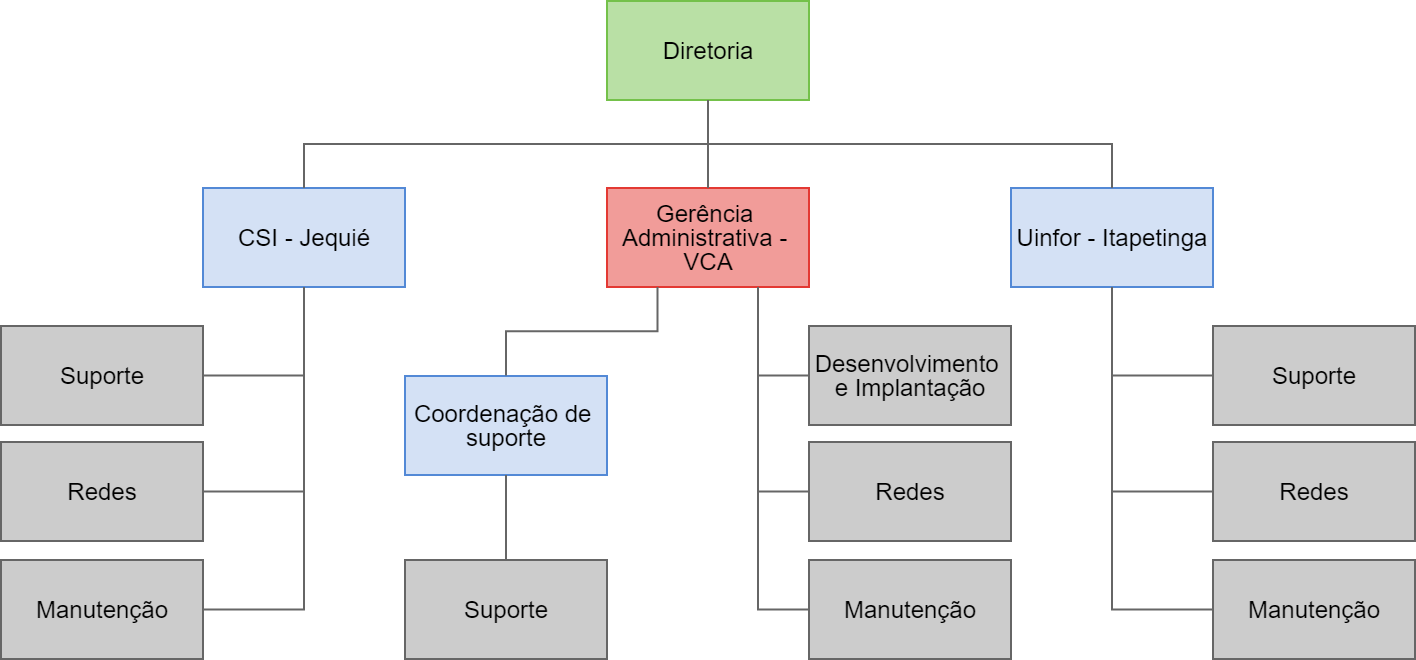
\includegraphics[scale=0.32]{imagens/organograma.png}
    \end{center}
    \FonteFigura{Roteiro de Diagnóstico Setorial.}
\end{figure}

\begin{itemize}
    \item Manutenção: realiza atividades como formatação e instalação de sistemas operacionais e outros softwares, troca de peças defeituosas, concerto de equipamentos com problemas, entre outras atividades relacionada aos equipamentos de informática.
    \item Redes: responsável por serviços de configuração da rede sem fio e com fio, implementação do cabeamento estruturado, configuração dos equipamentos de rede como roteadores, \textit{switches} e pontos de acesso sem fio. No campos de Vitória da Conquista o setor executa algumas atividades mais avançadas, como o gerenciamento da infra estrutura do \textit{datacenter} da UESB. 
    \item Suporte: atua no suporte ao uso dos sistemas de informação da universidade.
    \item Coordenação de suporte: responsável pelo relacionamento técnico com as empresas dos sistemas SAGRES e Pergamum e com o programa Mais Futuro.
    \item Gerencia Administrativa do campus de Vitória da Conquista: auxilia nos processos administrativos em geral, gerenciamento de pessoal, atendimento ao público, controle dos contratos gerenciados pela UINFOR, entre outros.
    \item Diretoria: encarregado das atividades como: assessorar a reitoria na gestão das TIC's; coordenar as áreas operacionais dos três campi; realizar o planejamento de aquisição de equipamentos e serviços de TIC's; emitir pareceres técnicos para subsidiar decisões da procuradoria jurídica e dos setores de licitações; e elaborar projetos juntamente com a AGESPI que visam financiar as TIC's.
\end{itemize}

\section{Avaliação da aplicação da TI Verde na UESB}

Com a aplicação do questionário, foi constatado que os seguintes fatores estão abaixo da média apresentada por \citeonline{lunardi2014desenvolvimento}: 
\begin{itemize}
    \item \textbf{Consciência socioambiental:} Existe falta de estratégias e políticas ambientais e para a utilização de recursos naturais como água, luz e papel. Apesar de frequentemente procurar parceiros comerciais que têm preocupações ambientais, a UESB só em algumas vezes pode ser considerada ambientalmente sustentável; 
    \item \textbf{Monitoramento:} Frequentemente controla os custos com manutenção dos equipamentos computacionais, mas em poucas ocasiões faz o gerenciamento do consumo de energia e o desempenho do mesmo;
    \item \textbf{Orientação ambiental:} Embora frequentemente incentive a reciclagem e faça recomendações aos funcionários de como economizar os produtos computacionais, falta uma preocupação com a conscientização dos funcionários, para que os mesmos apaguem a luz, utilizem o modo de descanso e desliguem os comutadores quando não estão em uso.
\end{itemize}

Já os seguintes fatores estão na média ou acima dela:

\begin{itemize}
    \item \textbf{\textit{Expertise} ambiental:} Foi verificado que a UINFOR possui um grande conhecimento sobre como diferentes tecnologias computacionais podem funcionar de forma mais eficiente e quais estão disponíveis no mercado. Ela também recorre a diferentes fontes para identificar tendencias mais limpas e econômicas e busca novas formas de redução do consumo de energia dos produtos computacionais como computadores, servidores e \textit{datacenters}. Em contrapartida, novamente foi verificado a falta de conscientização dos funcionários, sobre o uso racional dos recursos computacionais. 
    \item \textbf{Ações sustentáveis:} Fator em que a UINFOR mais se destaca, aplicando diferentes estratégias para melhor utilização dos produtos computacionais, removendo equipamentos computacionais que não estão em uso e fazendo suas últimas aquisições tecnológicas levando em consideração a eficiência energética. O único ponto abaixo foi o fato de como a grande maioria dos computadores da UESB foram adquiridos anos atrás, eles atualmente não são eficientes em termos de energia.
\end{itemize}

Com base na análise da entrevista realizada, do questionário aplicado e dos documentos lidos, pode-se compreender alguns pontos importantes para a pesquisa. Atualmente a UINFOR/UESB não possui estratégias e políticas ambientais bem definidas, embora utilize algumas práticas sustentáveis, que na maioria das vezes são utilizadas visando à economia e redução de gastos, se encaixando no primeiro nível das práticas da TI Verde, o TI Verde Tático. A seguir estes pontos são apresentados. 

A coleta, armazenamento e descarte dos REEE são realizadas da seguinte forma: Quando algum departamento detecta qualquer problema em algum equipamento eletroeletrônico, é aberto um chamado e o setor de manutenção realiza a busca do equipamento, os resíduos gerados pela manutenção são encaminhados para o almoxarifado, de lá os resíduos são enviados para uma central em Salvador, está central que realiza o processo de descarte, mas este processo é desconhecido pela UINFOR.

Na hora da aquisição de novos equipamentos, os selos Energy Star e RoHS são exigidos nas licitações realizadas. A equipe não possuí o conhecimentos dos 5 R's da sustentabilidade, embora seja levada a reduzir e reutilizar por conta da falta de verba.

Na opinião do diretor da UINFOR, a UESB precisa de estratégias para o consumo de água e de energia, além da utilização de um sistema de energia de 48 \textit{volts} para o \textit{datacenter} e a utilização de Computadores de Placa Única, para melhorar a sua sustentabilidade ambiental.

As principais práticas de TI Verde que a UINFOR utiliza são a Virtualização e o Gerenciamento Eletrônico de Documentos, explicadas a seguir.

A Virtualização tem como benefício a economia de gastos com hardware e a otimização do parque de servidores. Ela é utilizada para o compartilhamento de dezenas de servidores físicos, facilitando a administração e a otimização dos recursos. Ela é feita através do uso do programa \textit{VMware}. 

Já quanto ao Gerenciamento Eletrônico de Documentos, foi identificado que até então a UESB utilizava o sistema Lúpus, desenvolvido pela própria UESB. O Lúpus era responsável pela tramitação dos processos da UESB, mas ele está sendo descontinuado e sendo migrado para o Sistema Eletrônico de Informação (SEI). Outra aplicação é através do projeto de Gestão Eletrônica de Documentos.

\subsection{Projeto de Gestão Eletrônica de Documentos}

Para um melhor entendimento e compreensão do projeto, foi realizada uma entrevista com o analista e desenvolvedor do projeto no dia 14 de junho de 2014, utilizando o editor de texto online Google Documentos.

O projeto de GED tem como piloto o setor de Recursos Humanos (RH), é implementado através da modificação do software livre Alfresco, são utilizadas técnicas e padrões para recebimento, preparação, digitalização, indexação em software e disponibilização do acesso aos documentos por um meio digital. Ele tem como objetivos centralizar as fontes de informação da UESB, aumentar a acessibilidade à informação e armazenar os arquivos físicos de forma adequada.

A principal motivação do projeto piloto de GED, na área de RH, foi a opinião da equipe do setor, demonstrada através de uma consulta interna, indicando os prontuários físicos como a fonte mais confiável de informações. Através deste levantamento, foi decidido o investimento na digitalização e disponibilização dos documentos via ferramenta de software.

O projeto foi idealizado em 2011, inicialmente, buscando a terceirização da demanda. A partir de 2013, o Setor de Informações Funcionais assumiu a implantação do projeto. Atualmente ele está funcionando na Assessoria de Gestão de Pessoas (APG) e no Posto de Cadastro de Fornecedores (PCF), e se encontra em fase de análise/implantação na Reitoria e no Centro Universitário de Atenção à Saúde (CEUAS). 

O projeto tem caráter de aplicação contínua, e é esperado um processo maduro de produção e/ou recepção de documentos, armazenamento, descarte e acesso eficiente às informações. Entre as principais conquistas, estão a formação de uma equipe com conhecimento na área de GED, o crescente reconhecimento por parte da UESB e uma base de dados/documentos cada vez mais robusta. 

O estado atual do projeto pode ser classificado como "híbrido", pelo fato de ainda se trabalhar com documentos tanto em papel como em meio digital. A maior parte dos documentos que já foram digitalizados são recebidos mensalmente pelo GED-RH. Mas, além destes, existem documentos que já existiam antes do início do projeto, que ainda não foram processados, o que depende de mais pessoal, equipamentos e espaço para ser feito.

\subsection{Sistema Eletrônico de Informação}

O SEI foi desenvolvido pelo Tribunal Regional Federal da 4ª Região (TRF4), sendo um sistema de gestão de processos e documentos arquivísticos eletrônicos. As principais características são a libertação do papel como suporte físico para documentos institucionais e o compartilhamento do conhecimento com atualização e comunicação de novos eventos em tempo real. Ele faz parte de uma iniciativa conjunta de órgãos e entidades de diversas esferas da Administração Pública, sendo um produto do projeto Processo Eletrônico Nacional (PEN), possibilitando melhorias como ganhos em agilidade, produtividade, transparência e satisfação do público usuário, além de uma redução de custos. Ele permite a produção, edição, assinatura e trâmite de documentos, suas principais facilidades são: Portabilidade; Acesso Remoto; Acesso de usuários externos; Controle de nível de acesso; Tramitação em múltiplas unidades; Funcionalidades específicas; e Sistema intuitivo.$^{[}$\footnote{Informações retiradas do Manual do Usuário SEI, Disponível em: \url{https://softwarepublico.gov.br/social/articles/0004/9746/sei-doc-usuario.pdf}.  Acessado em 24 de junho de 2018}$^{]}$

Segundo uma matéria divulgada pelo portal do SEI Bahia$^{[}$\footnote{SEI Bahia já gerou economia de 7,5 milhões de folhas de papel, Disponível em: \url{http://www.portalseibahia.saeb.ba.gov.br/noticias/2018-06-15/sei-bahia-ja-gerou-economia-de-75-milhoes-de-folhas-de-papel}.  Acessado em 24 de junho de 2018}$^{]}$ o governo baiano já deixou de consumir 7,5 milhões de folhas de papel desde a implantação do projeto, e segundo o secretário de Administração do Estado, Edelvido Góes, a partir do dia 1º de novembro de 2018, todos os processos do Estado deverão tramitar obrigatoriamente em meio eletrônico através do sistema. O sistema já se encontra em fase de implantação e treinamento na UESB.

\section{Propostas}